\chapter{Data Analysis}\label{chap:dataanlysis}
This project will examine whether there exists a cointegration relation between the four cryptocurrencies, namely Bitcoin (BTC), Ethereum (ETH), Solana (SOL), and Ripple (XRP). In this chapter a short introduction to data is given, and afterwards the data will be analyzed. This will be done with the use of visual interpretation of plots as well as statistical tests.

\section{Data Introduction}
The data, that has been used, can be found at Yahoo Finance \cite{Yahoo_Finance}. The data for this project consists of opening prices, the daily lowest prices, the daily highest price, and the closing prices all in USD. The chosen period is from 10th of December 2020 to 10th October 2024. These cryptocurrencies have been chosen on the basis, that they are the largest coins measured on market capitalization, and the fact that none of them are so called stable coins, which is a coin pegged to a FIAT currency. The data for these cryptocurrencies have adjusted such that only the closing prices are included. It has then been checked for NA values, of which there are none. The data is then split into two parts: a training set, which consists of the first $90\%$ of the data, and a validation set, which consists of the last $10\%$. The training set is used to train and fit various models. Furthermore, model validation will be performed upon this data set. The validation set has been used to examine the forecasting ability and accuracy of the models.\\
\section{Leveled Graph}
The four cryptocurrencies' closing prices in USD are plotted below over the time period of the training data.
 \begin{figure}[H]
   \centering
   \subfloat[][Bitcoin]{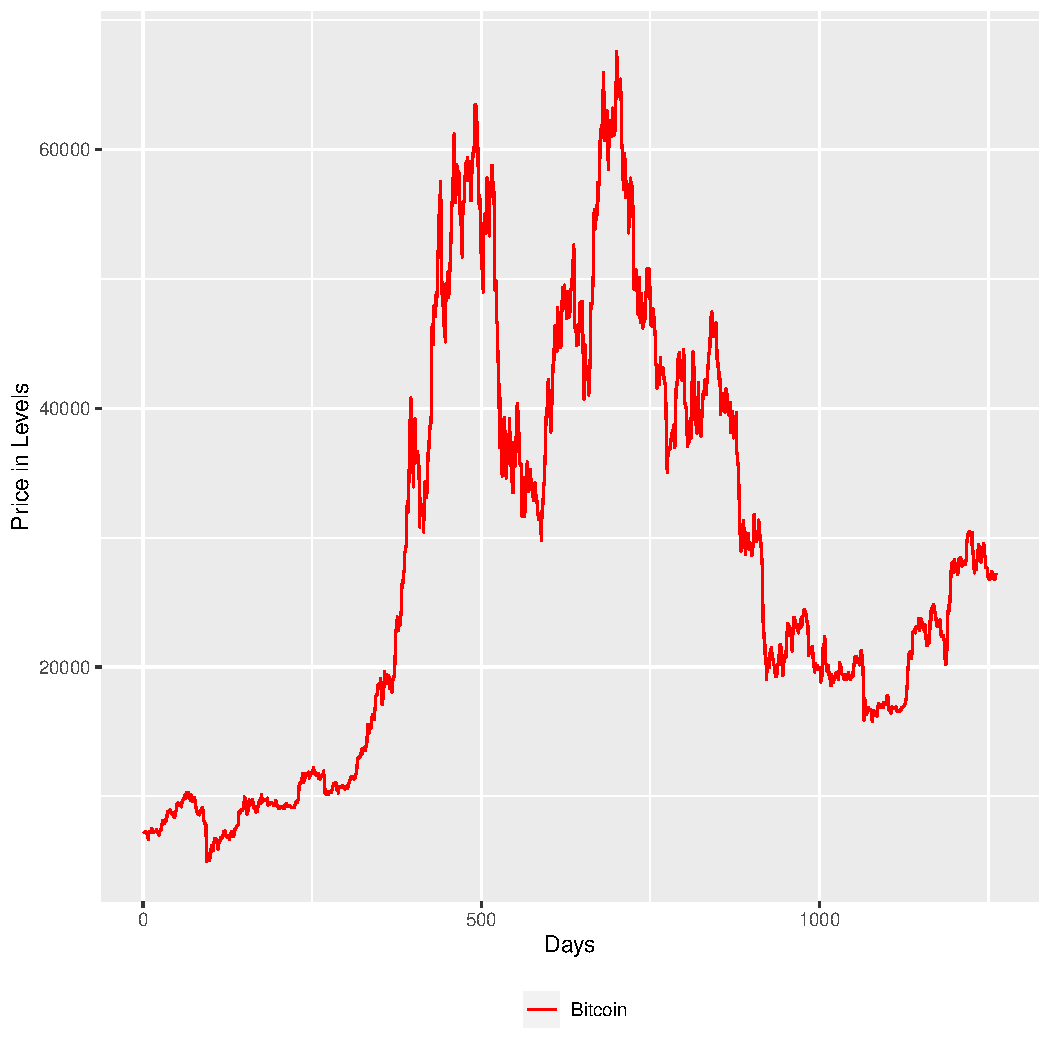
\includegraphics[width=.4\textwidth]{1.Projekt_kode/Billeder/Crypto_in_levels_Bitcoin.pdf}}\quad
   \subfloat[][Ethereum]{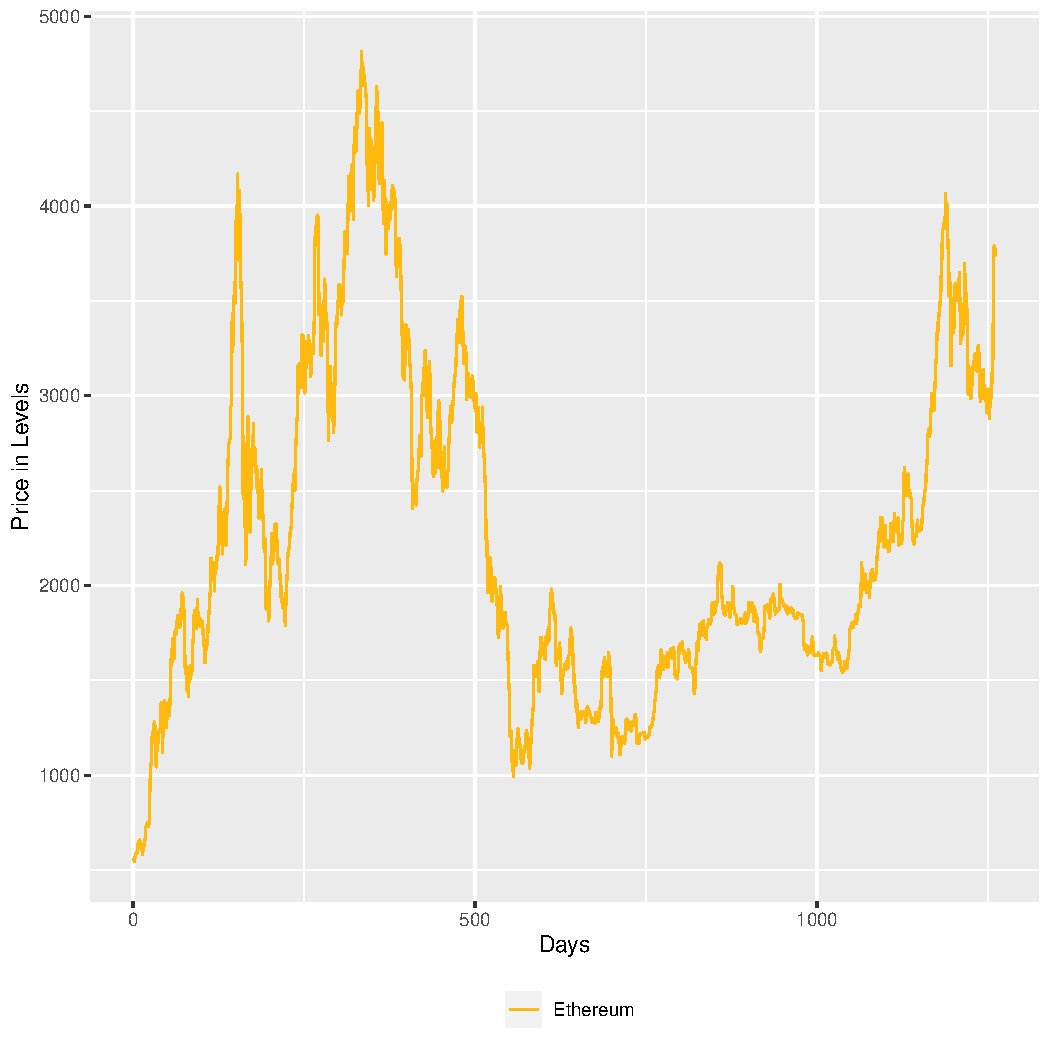
\includegraphics[width=.4\textwidth]{1.Projekt_kode/Billeder/Crypto_in_levels_Ethereum.pdf}}\\
   \subfloat[][Solana]{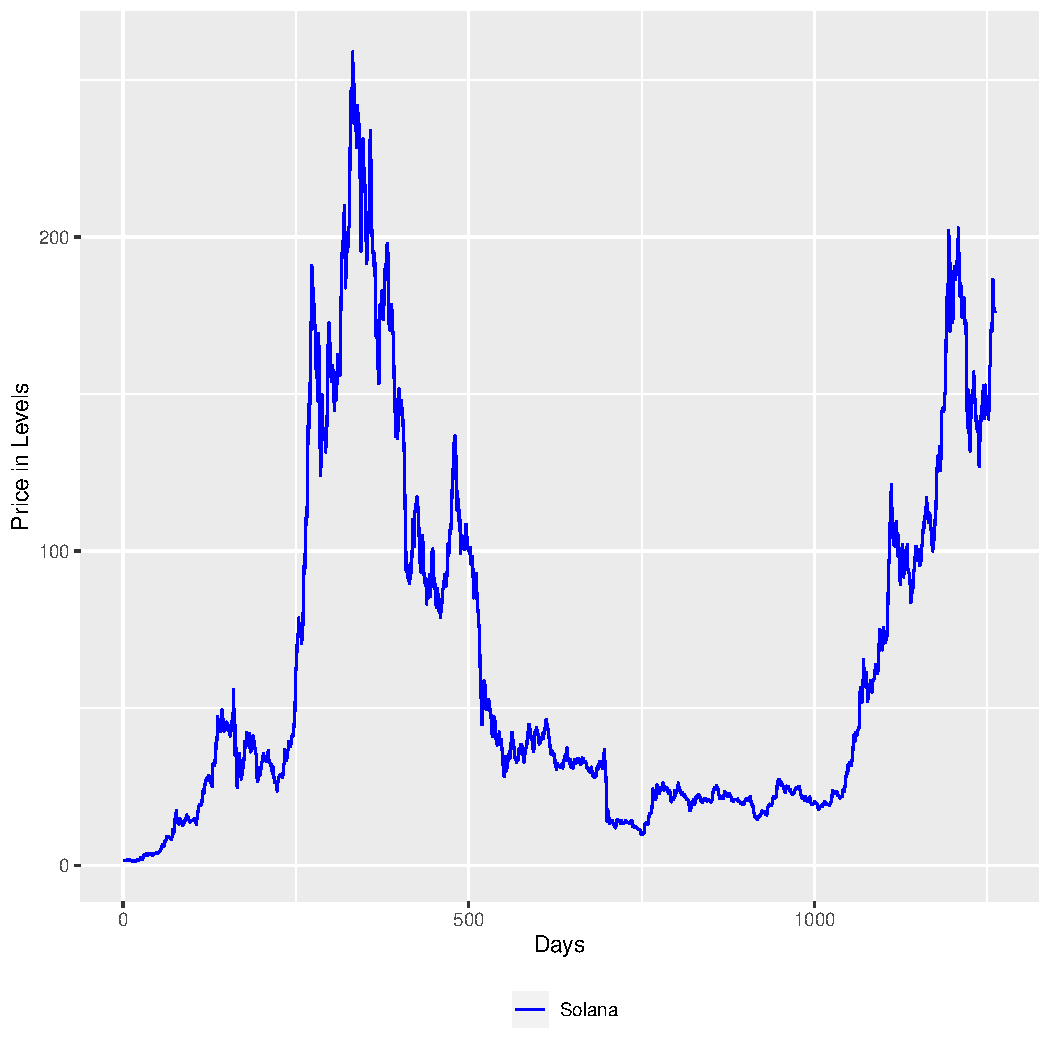
\includegraphics[width=.4\textwidth]{1.Projekt_kode/Billeder/Crypto_in_levels_Solana.pdf}}\quad
   \subfloat[][Ripple]{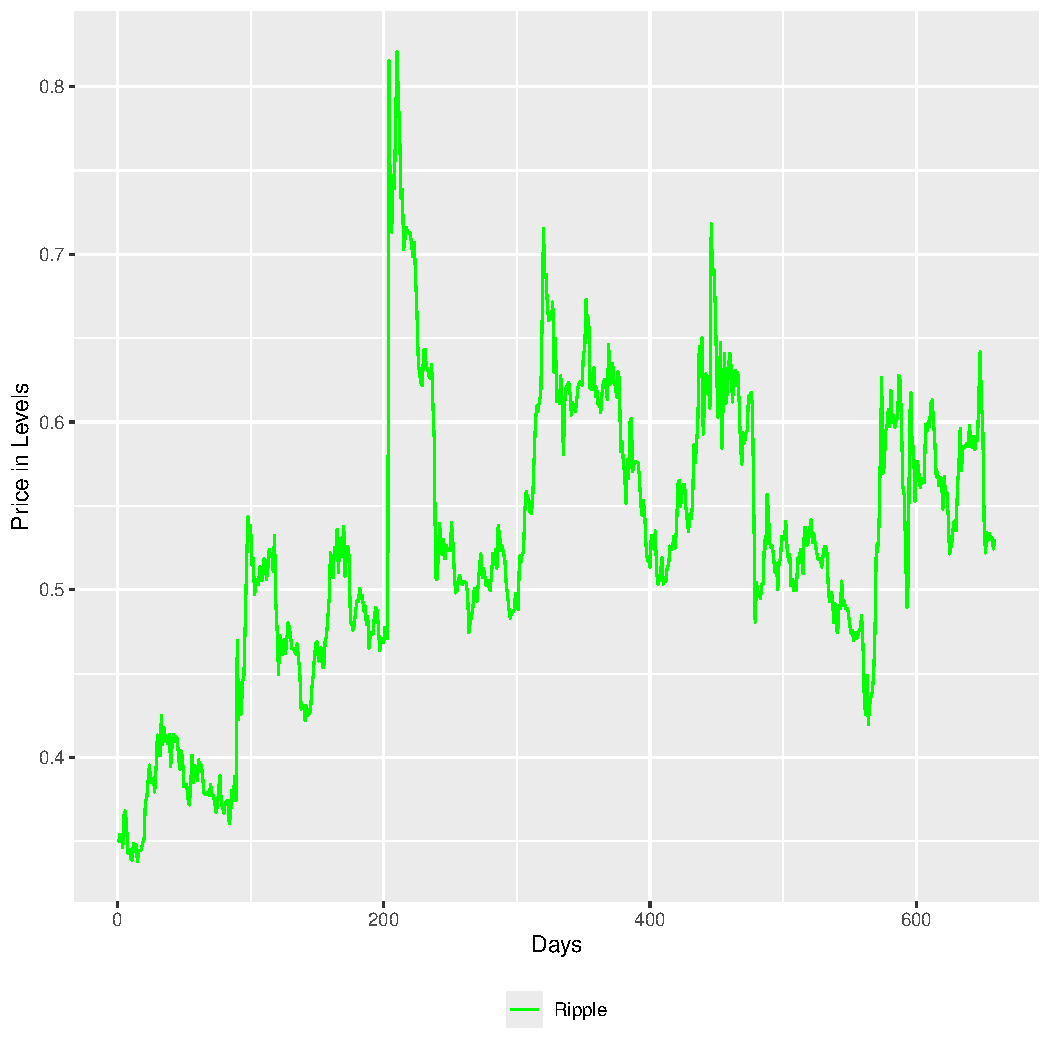
\includegraphics[width=.4\textwidth]{1.Projekt_kode/Billeder/Crypto_in_levels_Ripple.pdf}}
   \caption{Closing Prices in the Training Data}
   \label{graph_in_levels}
 \end{figure}
\noindent Initially the four plots in Figure \ref{graph_in_levels} exhibit a somewhat shared movement with a lot of similarities. One of these similarities is an explosive movement after day 1000 which is shared by BTC, ETH, and SOL. After reaching a peak a steep decline is followed. These joint movements emphasizes the theory of having some sort of cointegration movements.\\ 


\section{Model Validation}
For cointegration relations to exist, each time series must be non-stationary. Therefore, each time series will now be examined, in order to confirm that they are $I(1)$. Thus, each time series has been differenced using the R function \textit{diff}, and three graphs for each differenced time series have been made.
\begin{figure}[H]
  \centering
  \subfloat[][Bitcoin]{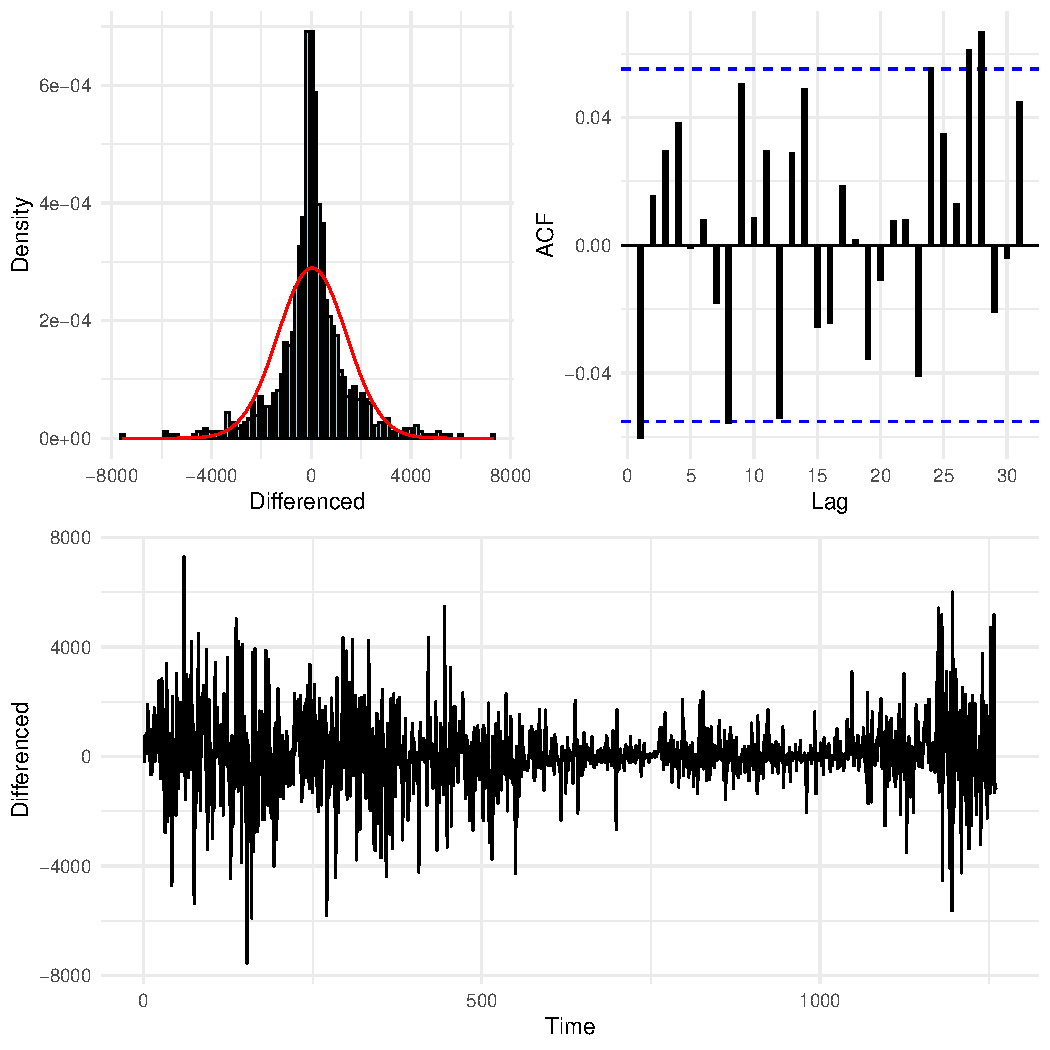
\includegraphics[width=.4\textwidth]{1.Projekt_kode/Billeder/plot_grid_Bitcoin.pdf}}\quad
  \subfloat[][Ethereum]{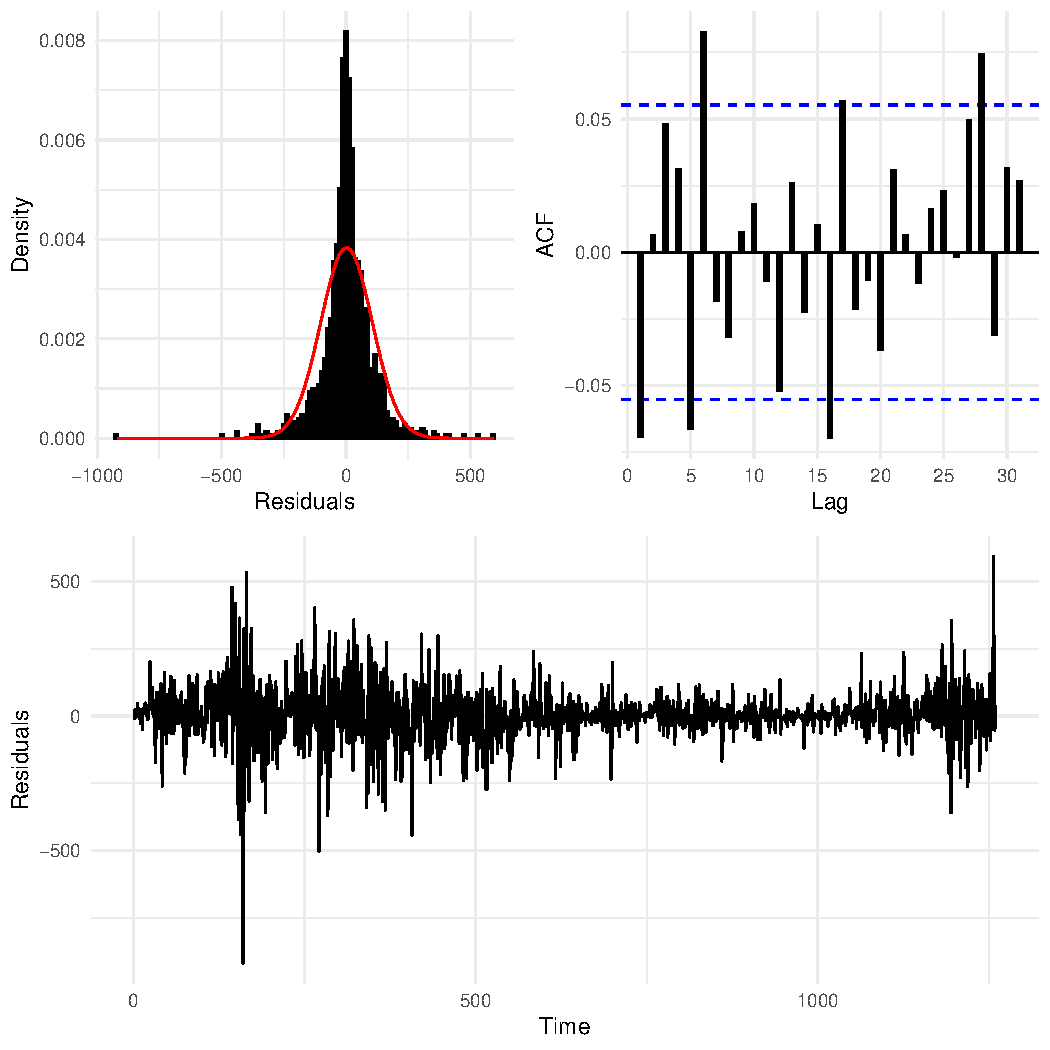
\includegraphics[width=.4\textwidth]{1.Projekt_kode/Billeder/plot_grid_Ethereum.pdf}}\\
  \subfloat[][Solana]{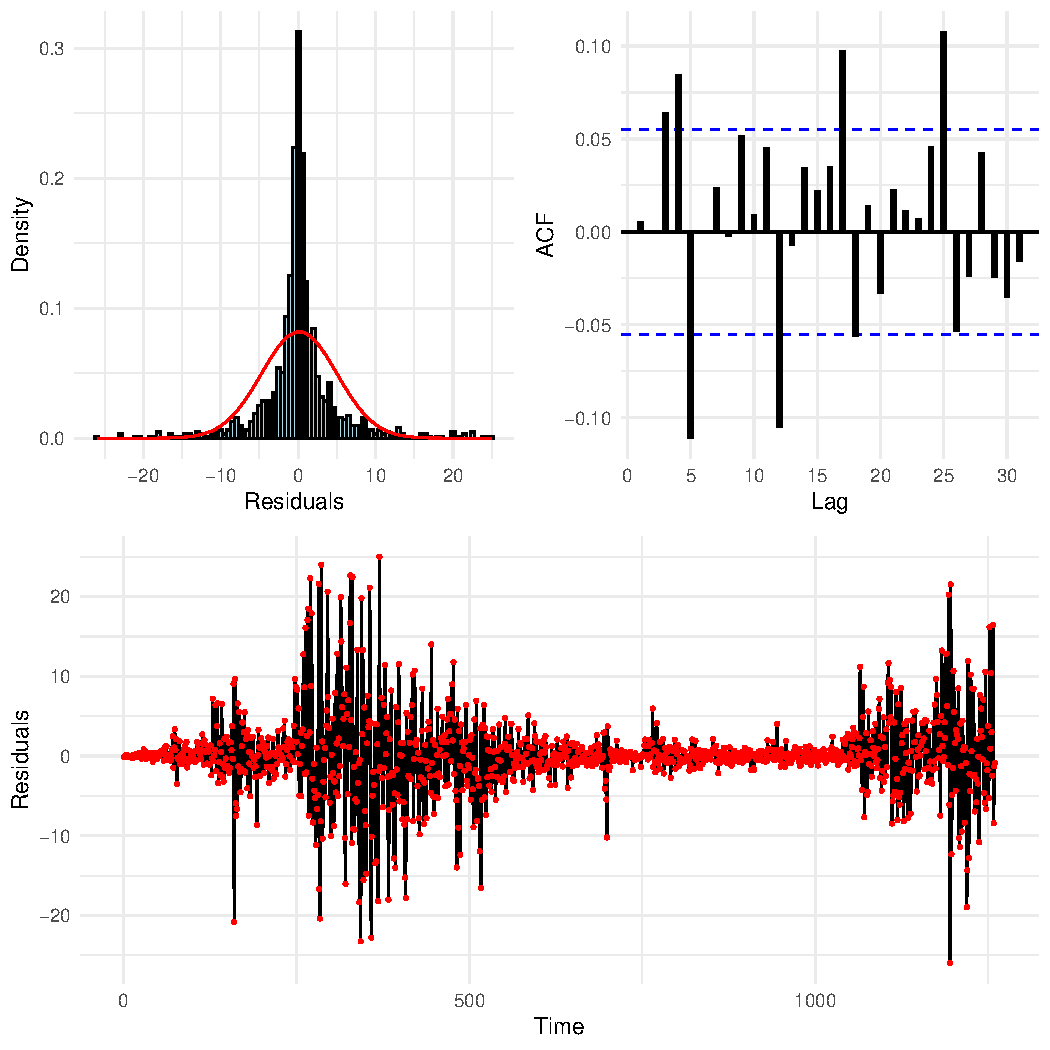
\includegraphics[width=.4\textwidth]{1.Projekt_kode/Billeder/plot_grid_Solana.pdf}}\quad
  \subfloat[][Ripple]{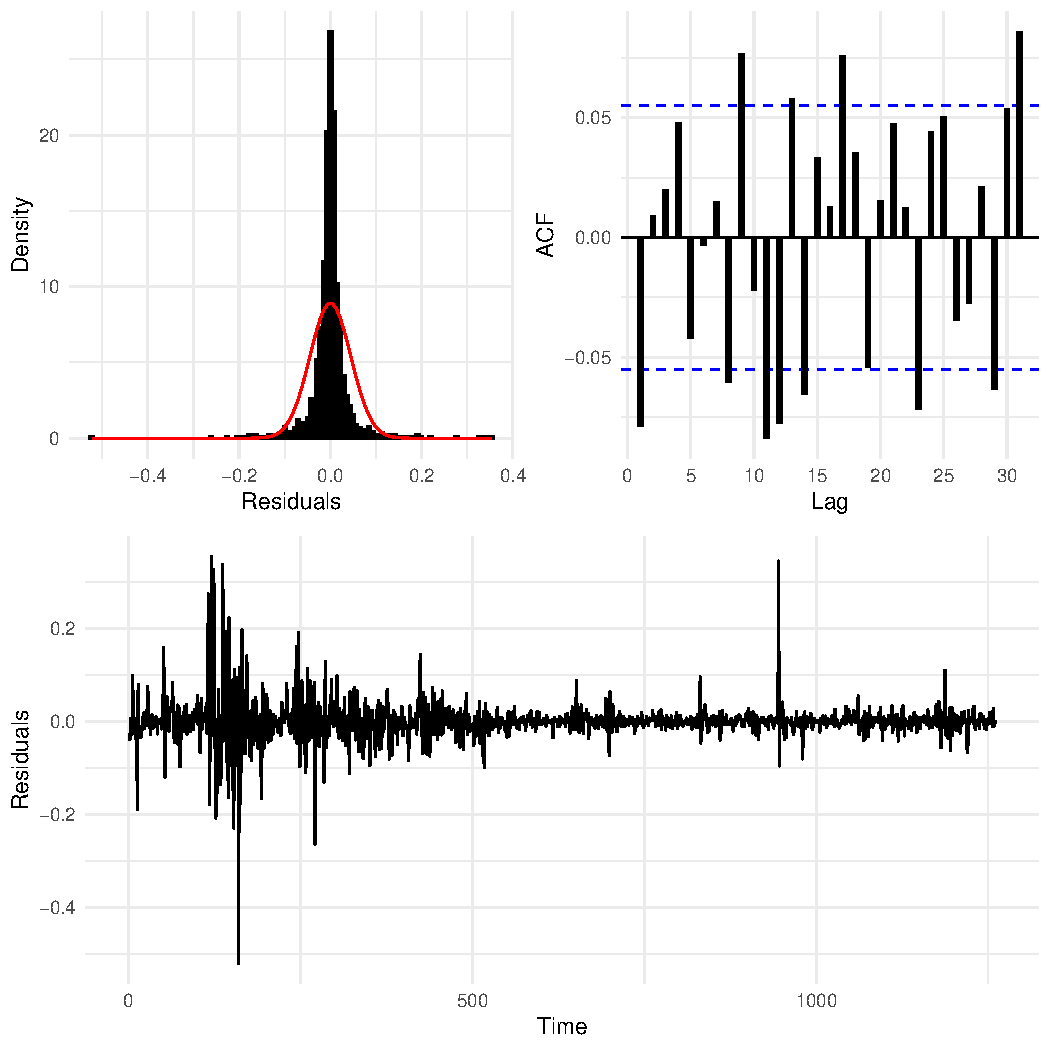
\includegraphics[width=.4\textwidth]{1.Projekt_kode/Billeder/plot_grid_Ripple.pdf}}
  \caption{Differenced data plots}
\end{figure}
\noindent The first of the three graphs in the top left is a histogram, from which it can be inferred that the data are evenly distributed around zero. The plot in the top right corner is an ACF plot, indicating stationary data. In the last plot, the data seems to fluctuate evenly around zero, even though there are clear volatility clusterings. 
Since the graphs indicate stationary data, it can be assumed that all four time series are $I(1)$, which is supported by the results achieved by the R function \textit{adf.test}, which computes the Augmented Dickey Fuller.\\

\noindent Next, the residuals of the optimal \textit{VAR} model will be examined. First, the R function \textit{VARselect} will be used on the differenced data, which gives the optimal lag order based on four different criteria, namely AIC, HQ, BIC, and FPE. 
Here, the AIC is chosen since the AIC and BIC is preferred when forecasting. There are incentives for choosing both an AIC and BIC, the BIC is preferred for large sample sizes, which is the case in this instance, but in hindsight the BIC generally chooses a less complicated model since it penalizes extra parameters more than the AIC. This, in unison with the fact that the BIC is often advantageous when the true model is present, which can not be assumed, leads us to believe the AIC is more efficient \cite{AICorBIC}. The AIC is computed as:
\begin{equation*}
    AIC=2k-2ln(L)
\end{equation*}
Where $k$ is the number of parameters and $L$ is the likelihood function. The maximum lag is chosen to be $10$, since there is no desire to over complicate a model with an excessive amount of lags. The AIC score for one through ten is plotted below, where the ninth lag corresponds to the lowest value. The lag chosen is five, since the difference between the two is minimal, and, as mentioned before, fewer lags are preferred.
\begin{figure}[H]
    \centering
    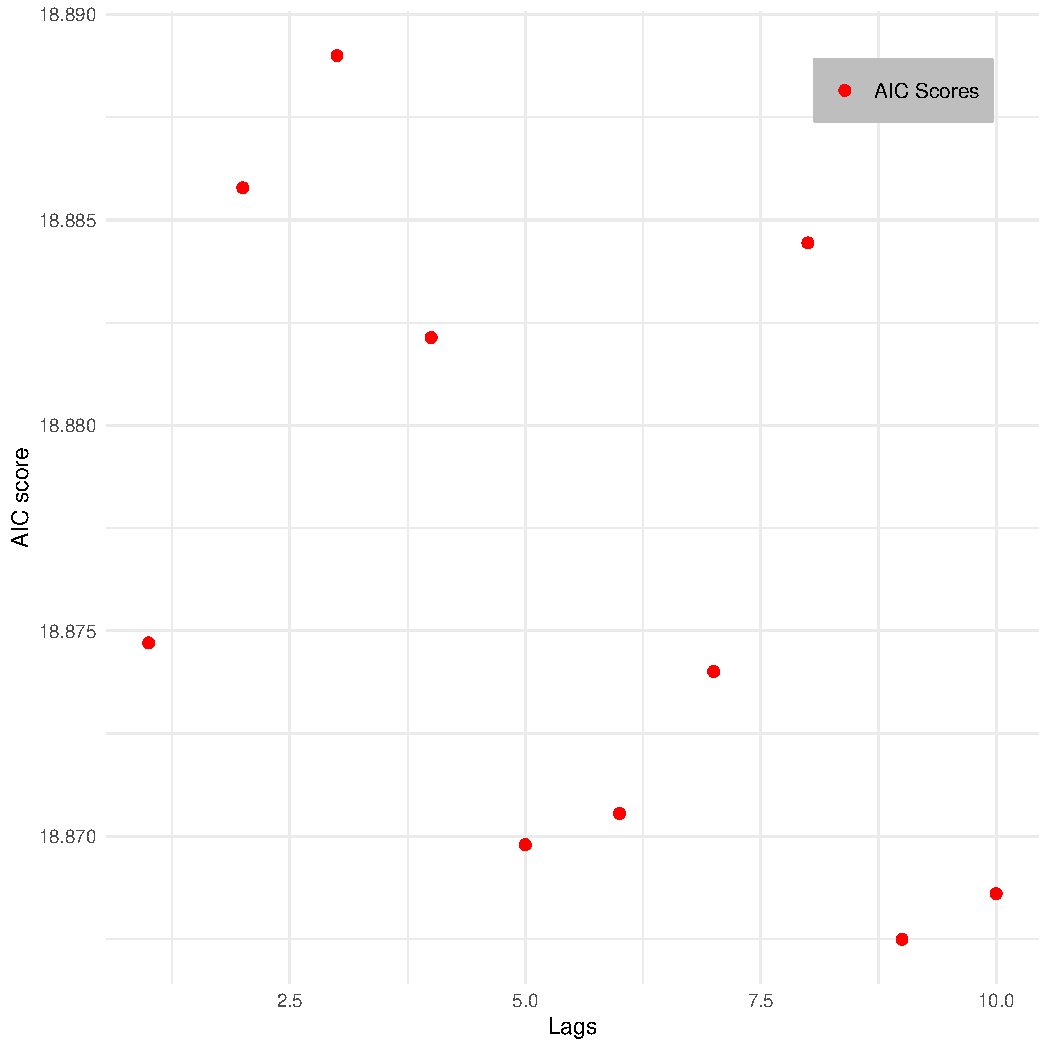
\includegraphics[width=0.5\linewidth]{1.Projekt_kode/Billeder/Crypto_lags.pdf}
    \caption{AIC values lag one through ten}
\end{figure}
\noindent The R function \textit{VAR} is used, with the lag order specified to five, thus a \textit{VAR}$(5)$ model is produced, the coefficients can be found in Appendix \ref{app:Var_estimations}. Next the R function \textit{checkresiduals} is applied to the residuals of each currency. It produces both the plots in Figure \ref{fig:plot_over_residuals} and the Ljung-Box test. The Ljung-Box test is a statistical tool used, to analyze if the errors exhibit an uncorrelated pattern. It has the test statistic 
\begin{align*}
    Q=T(T-2)\sum^H_{h=1}\frac{\hat{r}^2_{h}}{T-h}
\end{align*}
with $\hat{r}$ being the sample autocorrelations for standardized residuals, T the number of observations, and H arbitrarily chosen as the maximum amount of allowed lags. This statistic is compared against the $\chi^2$-distribution and rejects the null hypothesis, assuming the model does not exhibit a lack of fit, when
\begin{align*}
    Q>\chi^2_{1-\alpha,H-p-q}.
\end{align*}
\begin{table}[H]
\centering
\begin{tabular}{|l|c|c|c|}
\hline
\textbf{Cryptocurrency} & $\b{\chi^2}$ & \textbf{Degrees of Freedom} & \textbf{$p$-value} \\
\hline
BTC & 0.11156 & 5 & 0.9998 \\
ETH & 0.99379 & 5 & 0.9631 \\
SOL & 0.099654 & 5 & 0.9998 \\
XRP & 0.58619 & 5 & 0.9886 \\
\hline
\end{tabular}
\caption{Ljung-Box test results for cryptocurrency residuals}
\label{tab:ljung_box}
\end{table}
\noindent The large $p$-values indicate that the null hypothesis can not be rejected, thus indicating, no significant autocorrelation. This means the residuals does not exhibit significant dependence or autocorrelation up to lag five, which suggests that the models have captured the autocorrelation.
\begin{figure}[H]
  \centering
  \subfloat[][Bitcoin]{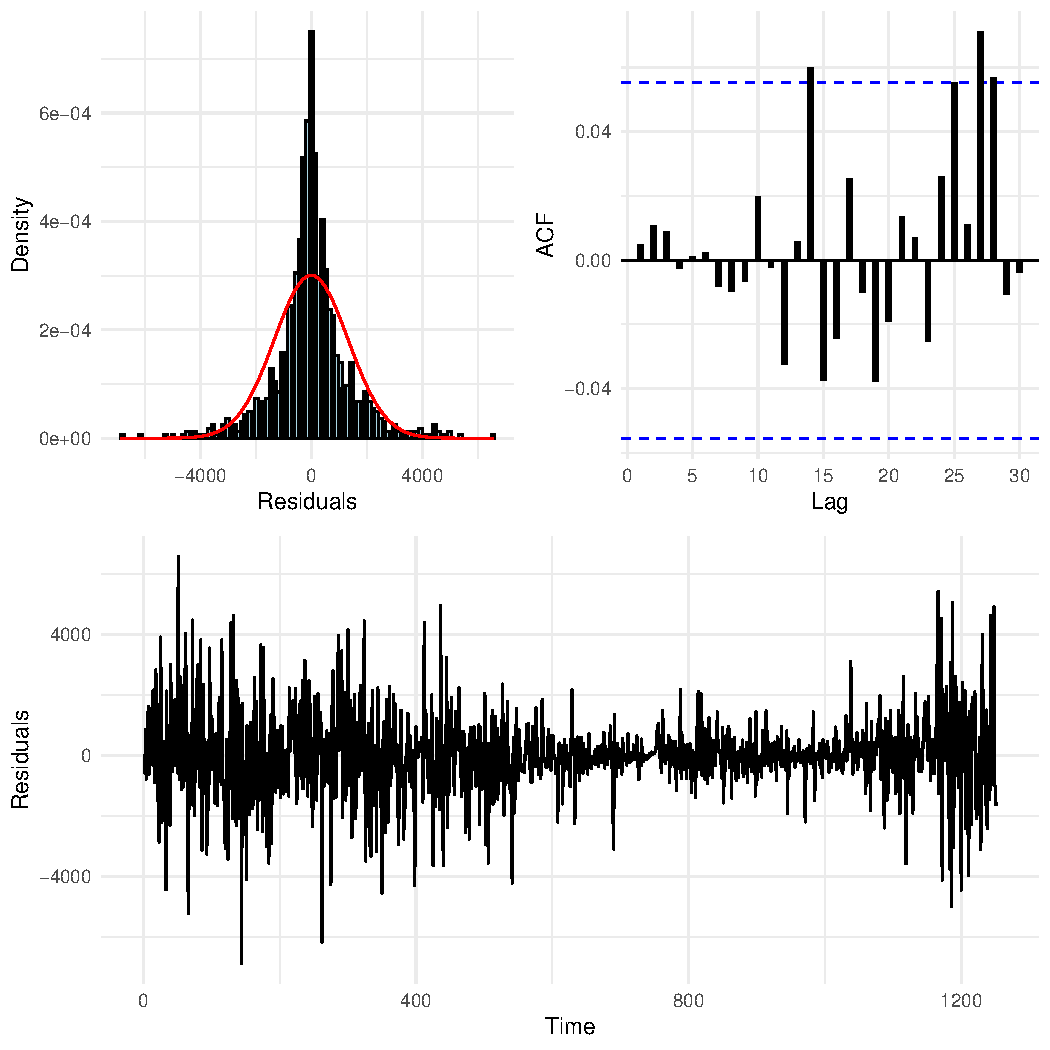
\includegraphics[width=.35\textwidth]{1.Projekt_kode/Billeder/plot_grid_ResidualsResiduals_BTC.pdf}}\quad
  \subfloat[][Ethereum]{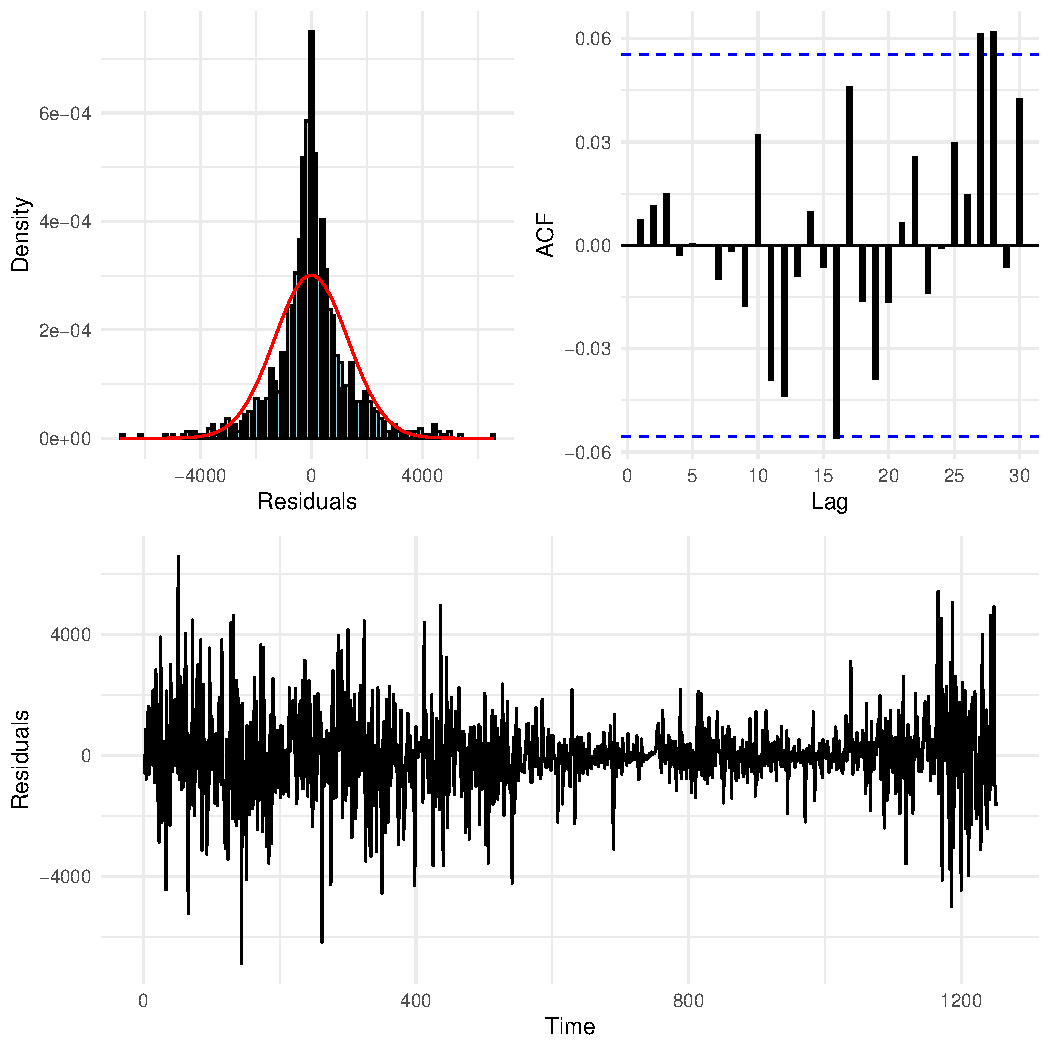
\includegraphics[width=.35\textwidth]{1.Projekt_kode/Billeder/plot_grid_ResidualsResiduals_ETH.pdf}}\\
  \subfloat[][Solana]{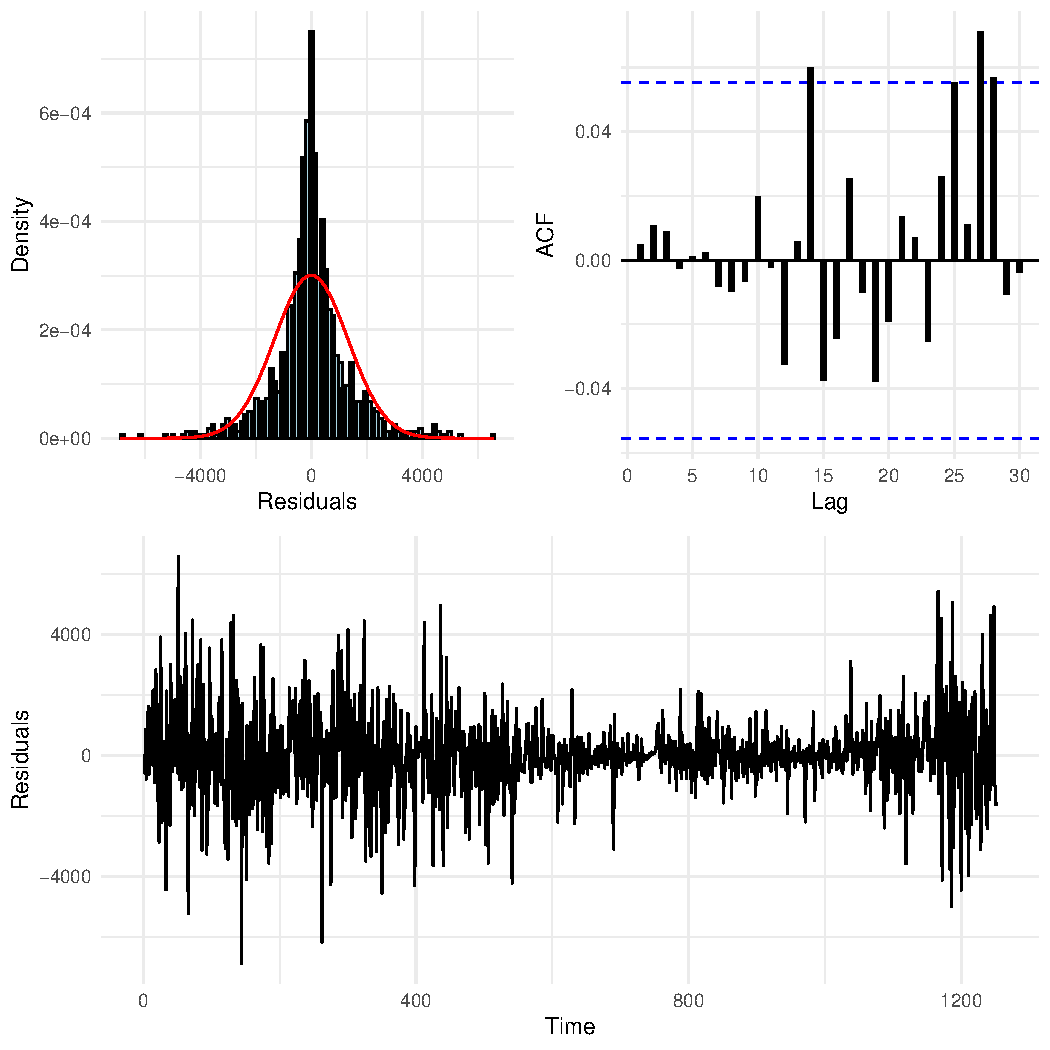
\includegraphics[width=.35\textwidth]{1.Projekt_kode/Billeder/plot_grid_ResidualsResiduals_SOL.pdf}}\quad
  \subfloat[][Ripple]{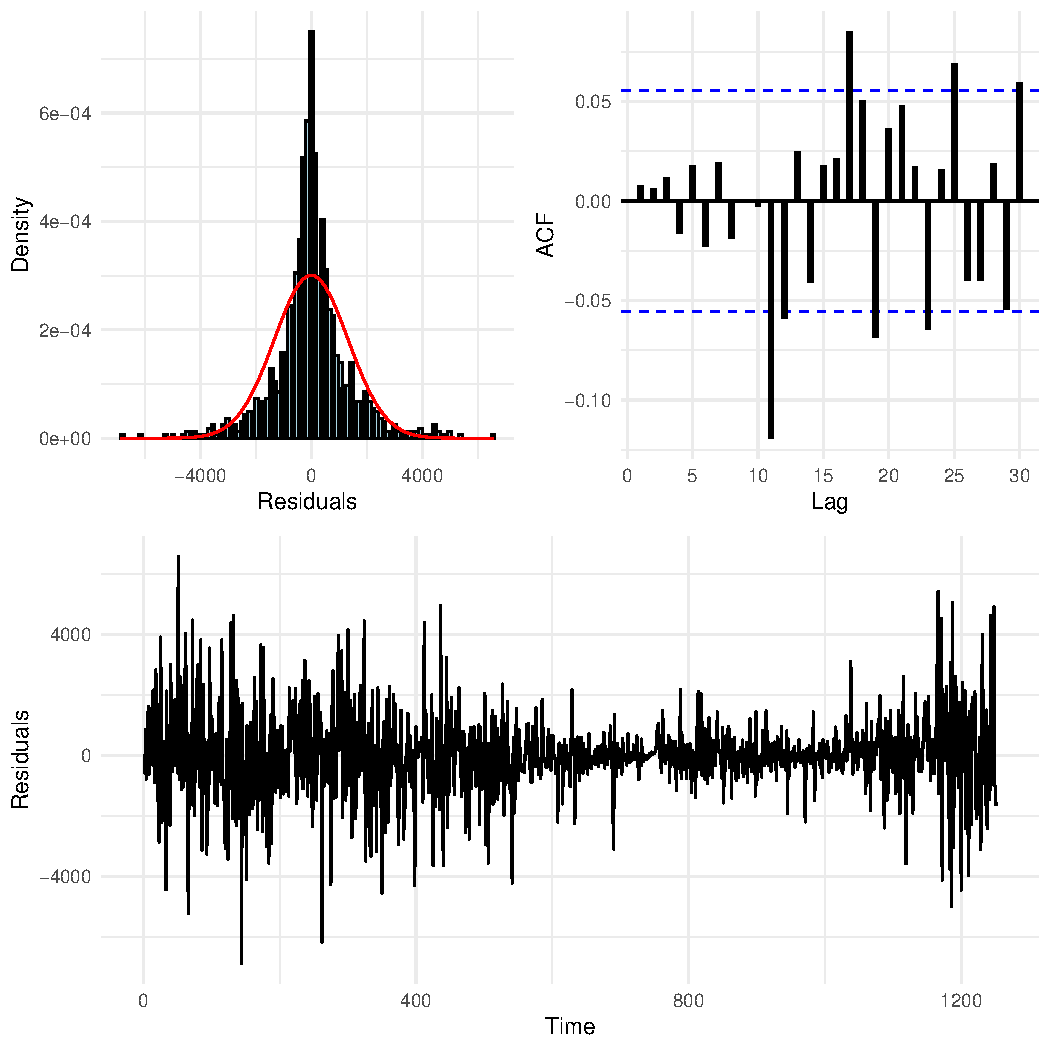
\includegraphics[width=.35\textwidth]{1.Projekt_kode/Billeder/plot_grid_ResidualsResiduals_XRP.pdf}}
  \caption{Different plots over the residuals}
  \label{fig:plot_over_residuals}
\end{figure}
\noindent The histograms seems to be somewhat normally distributed with mean zero, although there are many observations in the center, and some extreme values indicating heavy tales. This can also be emphasized in the residual plots, where it seems to oscillate around zero with some volatility clustering.
The ACF indicates stationary residuals.


\pause

\noindent Looking at the QQ-plots the desired tendency would be residuals following the red line, since that would indicate normality in the residuals. 
\begin{figure}[H]
  \centering
  \subfloat[][Bitcoin]{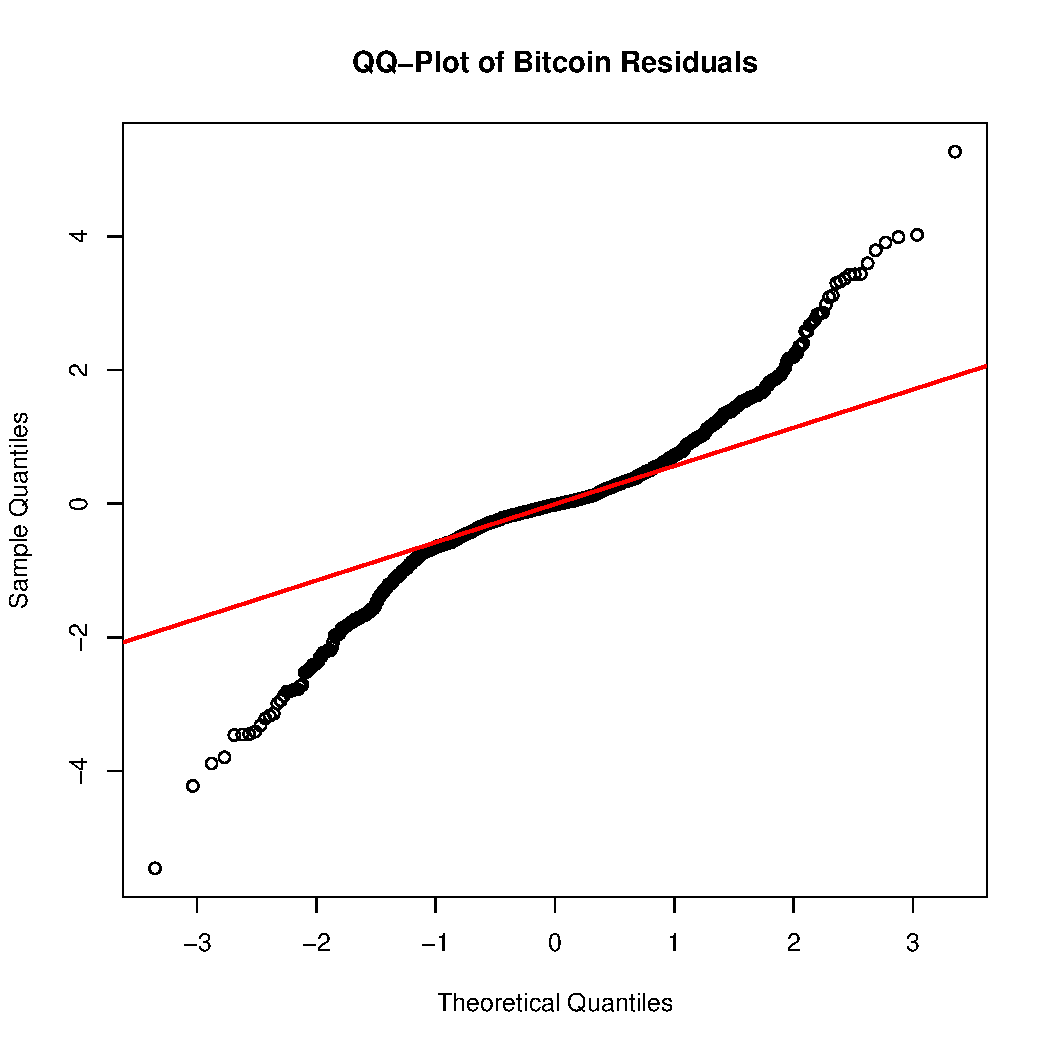
\includegraphics[width=.35\textwidth]{1.Projekt_kode/Billeder/QQ-Plot_of_Bitcoin_Residuals_plot.pdf}}\quad
  \subfloat[][Ethereum]{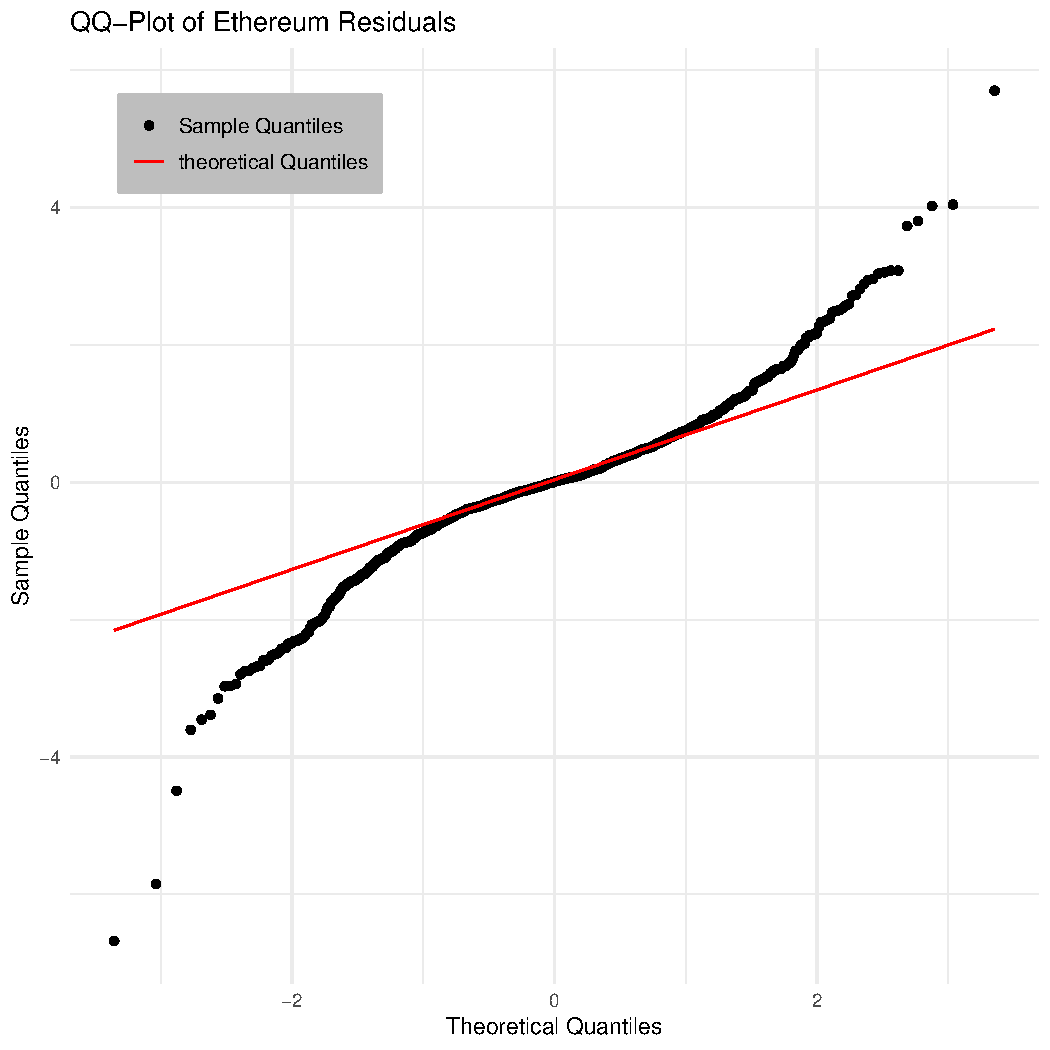
\includegraphics[width=.35\textwidth]{1.Projekt_kode/Billeder/QQ-Plot_of_Ethereum_Residuals_plot.pdf}}\\
  \subfloat[][Solana]{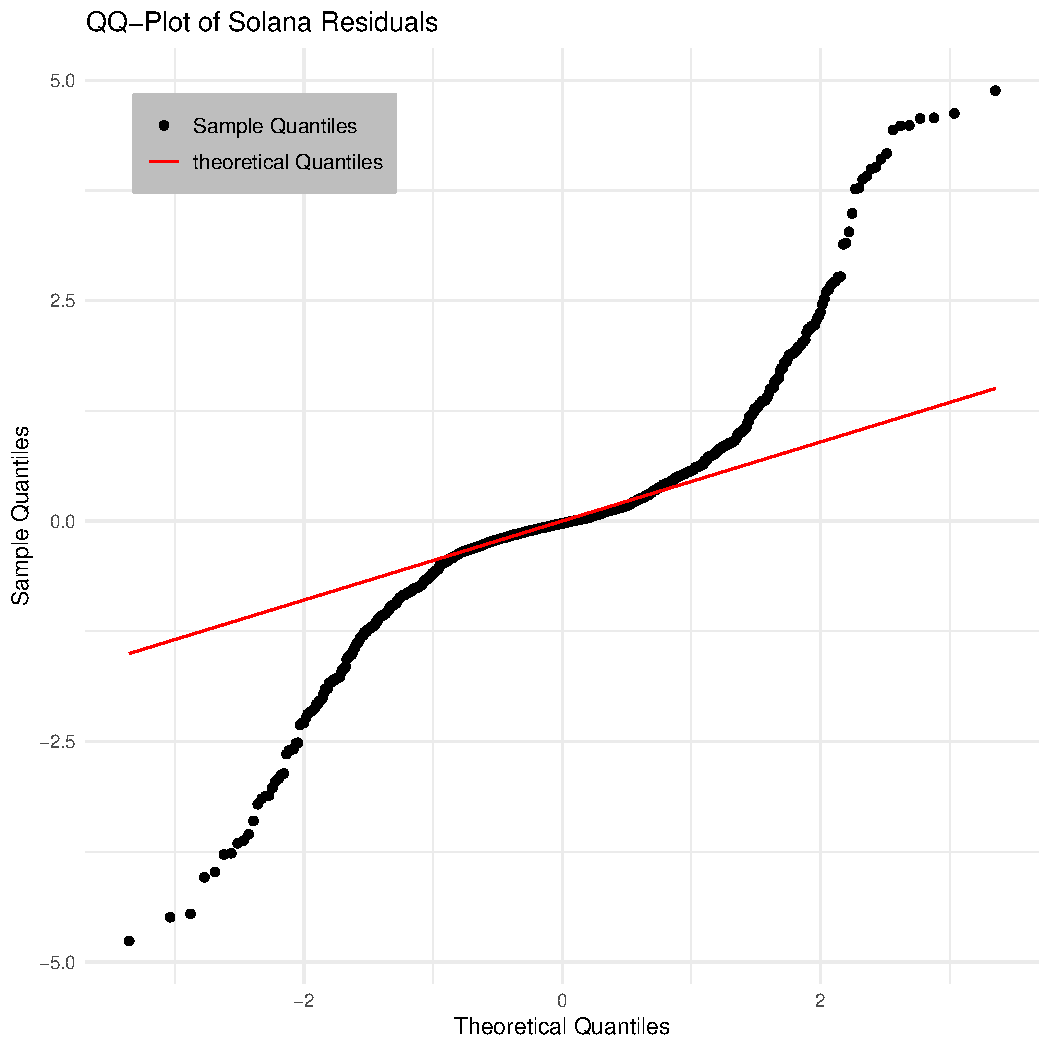
\includegraphics[width=.35\textwidth]{1.Projekt_kode/Billeder/QQ-Plot_of_Solana_Residuals_plot.pdf}}\quad
  \subfloat[][Ripple]{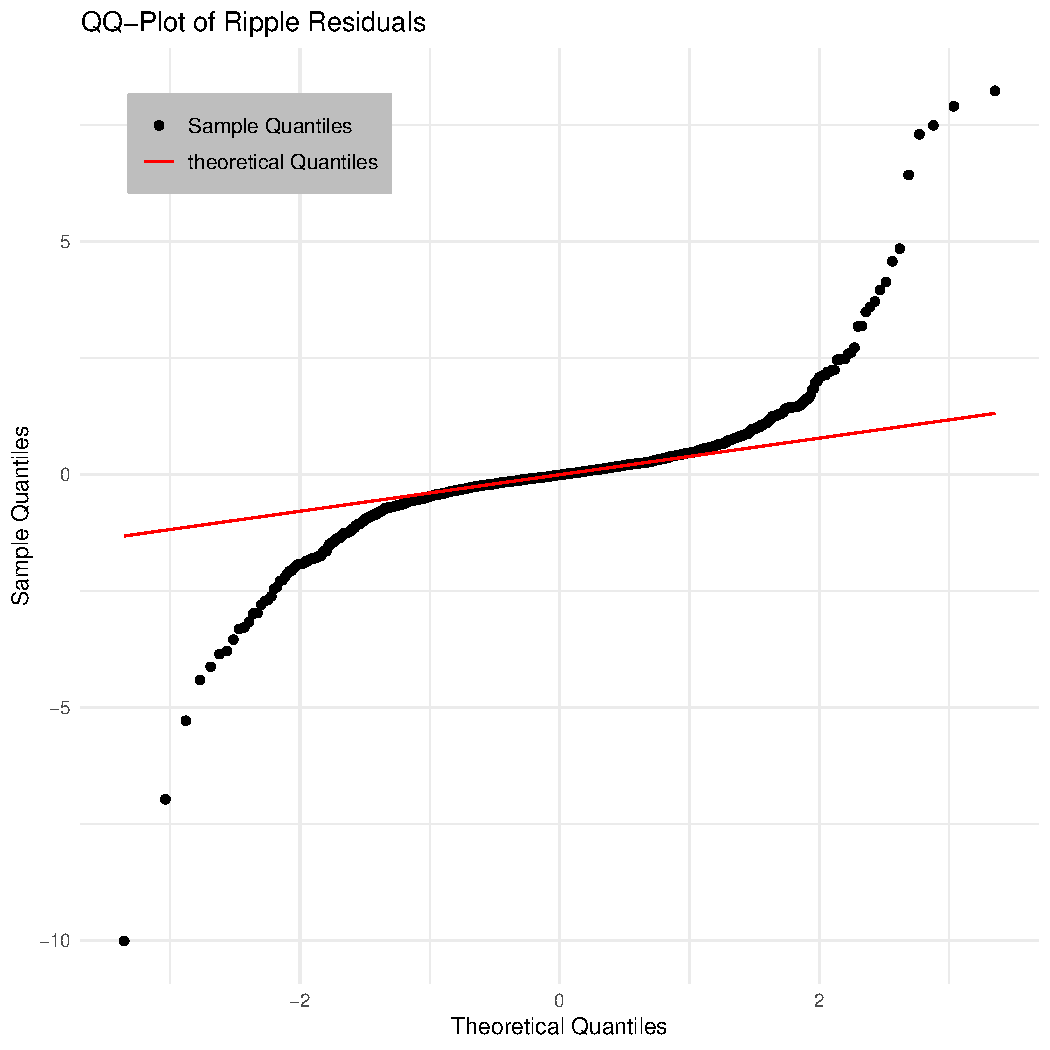
\includegraphics[width=.35\textwidth]{1.Projekt_kode/Billeder/QQ-Plot_of_Ripple_Residuals_plot.pdf}}
  \caption{QQ-plots}
\end{figure}
\noindent The normality assumption is questioned since the plots indicate heavy tales, meaning that they have more extreme values than a normal distribution. This bias can also be seen earlier in the histogram. Thus, the normality assumption is not necessarily fulfilled. The conclusions from the QQ-plots above are supported by the R function \textit{arch.test} and \textit{normality.test}, both of which reject the null hypothesis. This means that there is statistical incentive to assume that the residuals contain heteroscedasticity, and furthermore that there is no indication of normality. Even though this is the case, in order to continue the application, it will be assumed that the residuals are normal in unison with there being no heteroscedasticity in the residuals.